\documentclass{beamer} 
\usepackage[utf8]{inputenc}
\usepackage[T1]{fontenc}
\usepackage{lmodern}

\usetheme{default}
\setbeamertemplate{navigation symbols}{}
\setbeamertemplate{caption}[numbered] 
\graphicspath{{images/}}

\title{WIPS - Wireless Indoor Presence Sensing} 
\author{Erik Grafström, Max Morén, Erik Olsson} 
\date{May 31, 2011} 

\begin{document}

\begin{frame}
	\titlepage
\end{frame}

\begin{frame} 
\frametitle{Who we are}

	\begin{block}

		Erik Grafström

	\end{block}

	\begin{block}

		Max Morén
	
	\end{block}
	
	\begin{block}
	
		Erik Olsson

	\end{block}

\end{frame}

\begin{frame} 
\frametitle{Project areas}

	\begin{columns}

	\column{0.2\textwidth}

	\begin{block}

		\emph{W} - Wireless

	\end{block}

	\begin{block}

		\emph{I} - Indoor
	
	\end{block}
	
	\begin{block}
	
		\emph{P} - Presence

	\end{block}

	\begin{block}
	
		\emph{S} - Sensing

	\end{block}

	\column{0.8\textwidth}

	WIPS encompasses two of the proposed areas, \emph{Environmental monitoring} 
	and \emph{Network measurements and analysis}.
	
	\end{columns}

\end{frame} 

\begin{frame}
\frametitle{Project scenario}
	
	\begin{figure}
		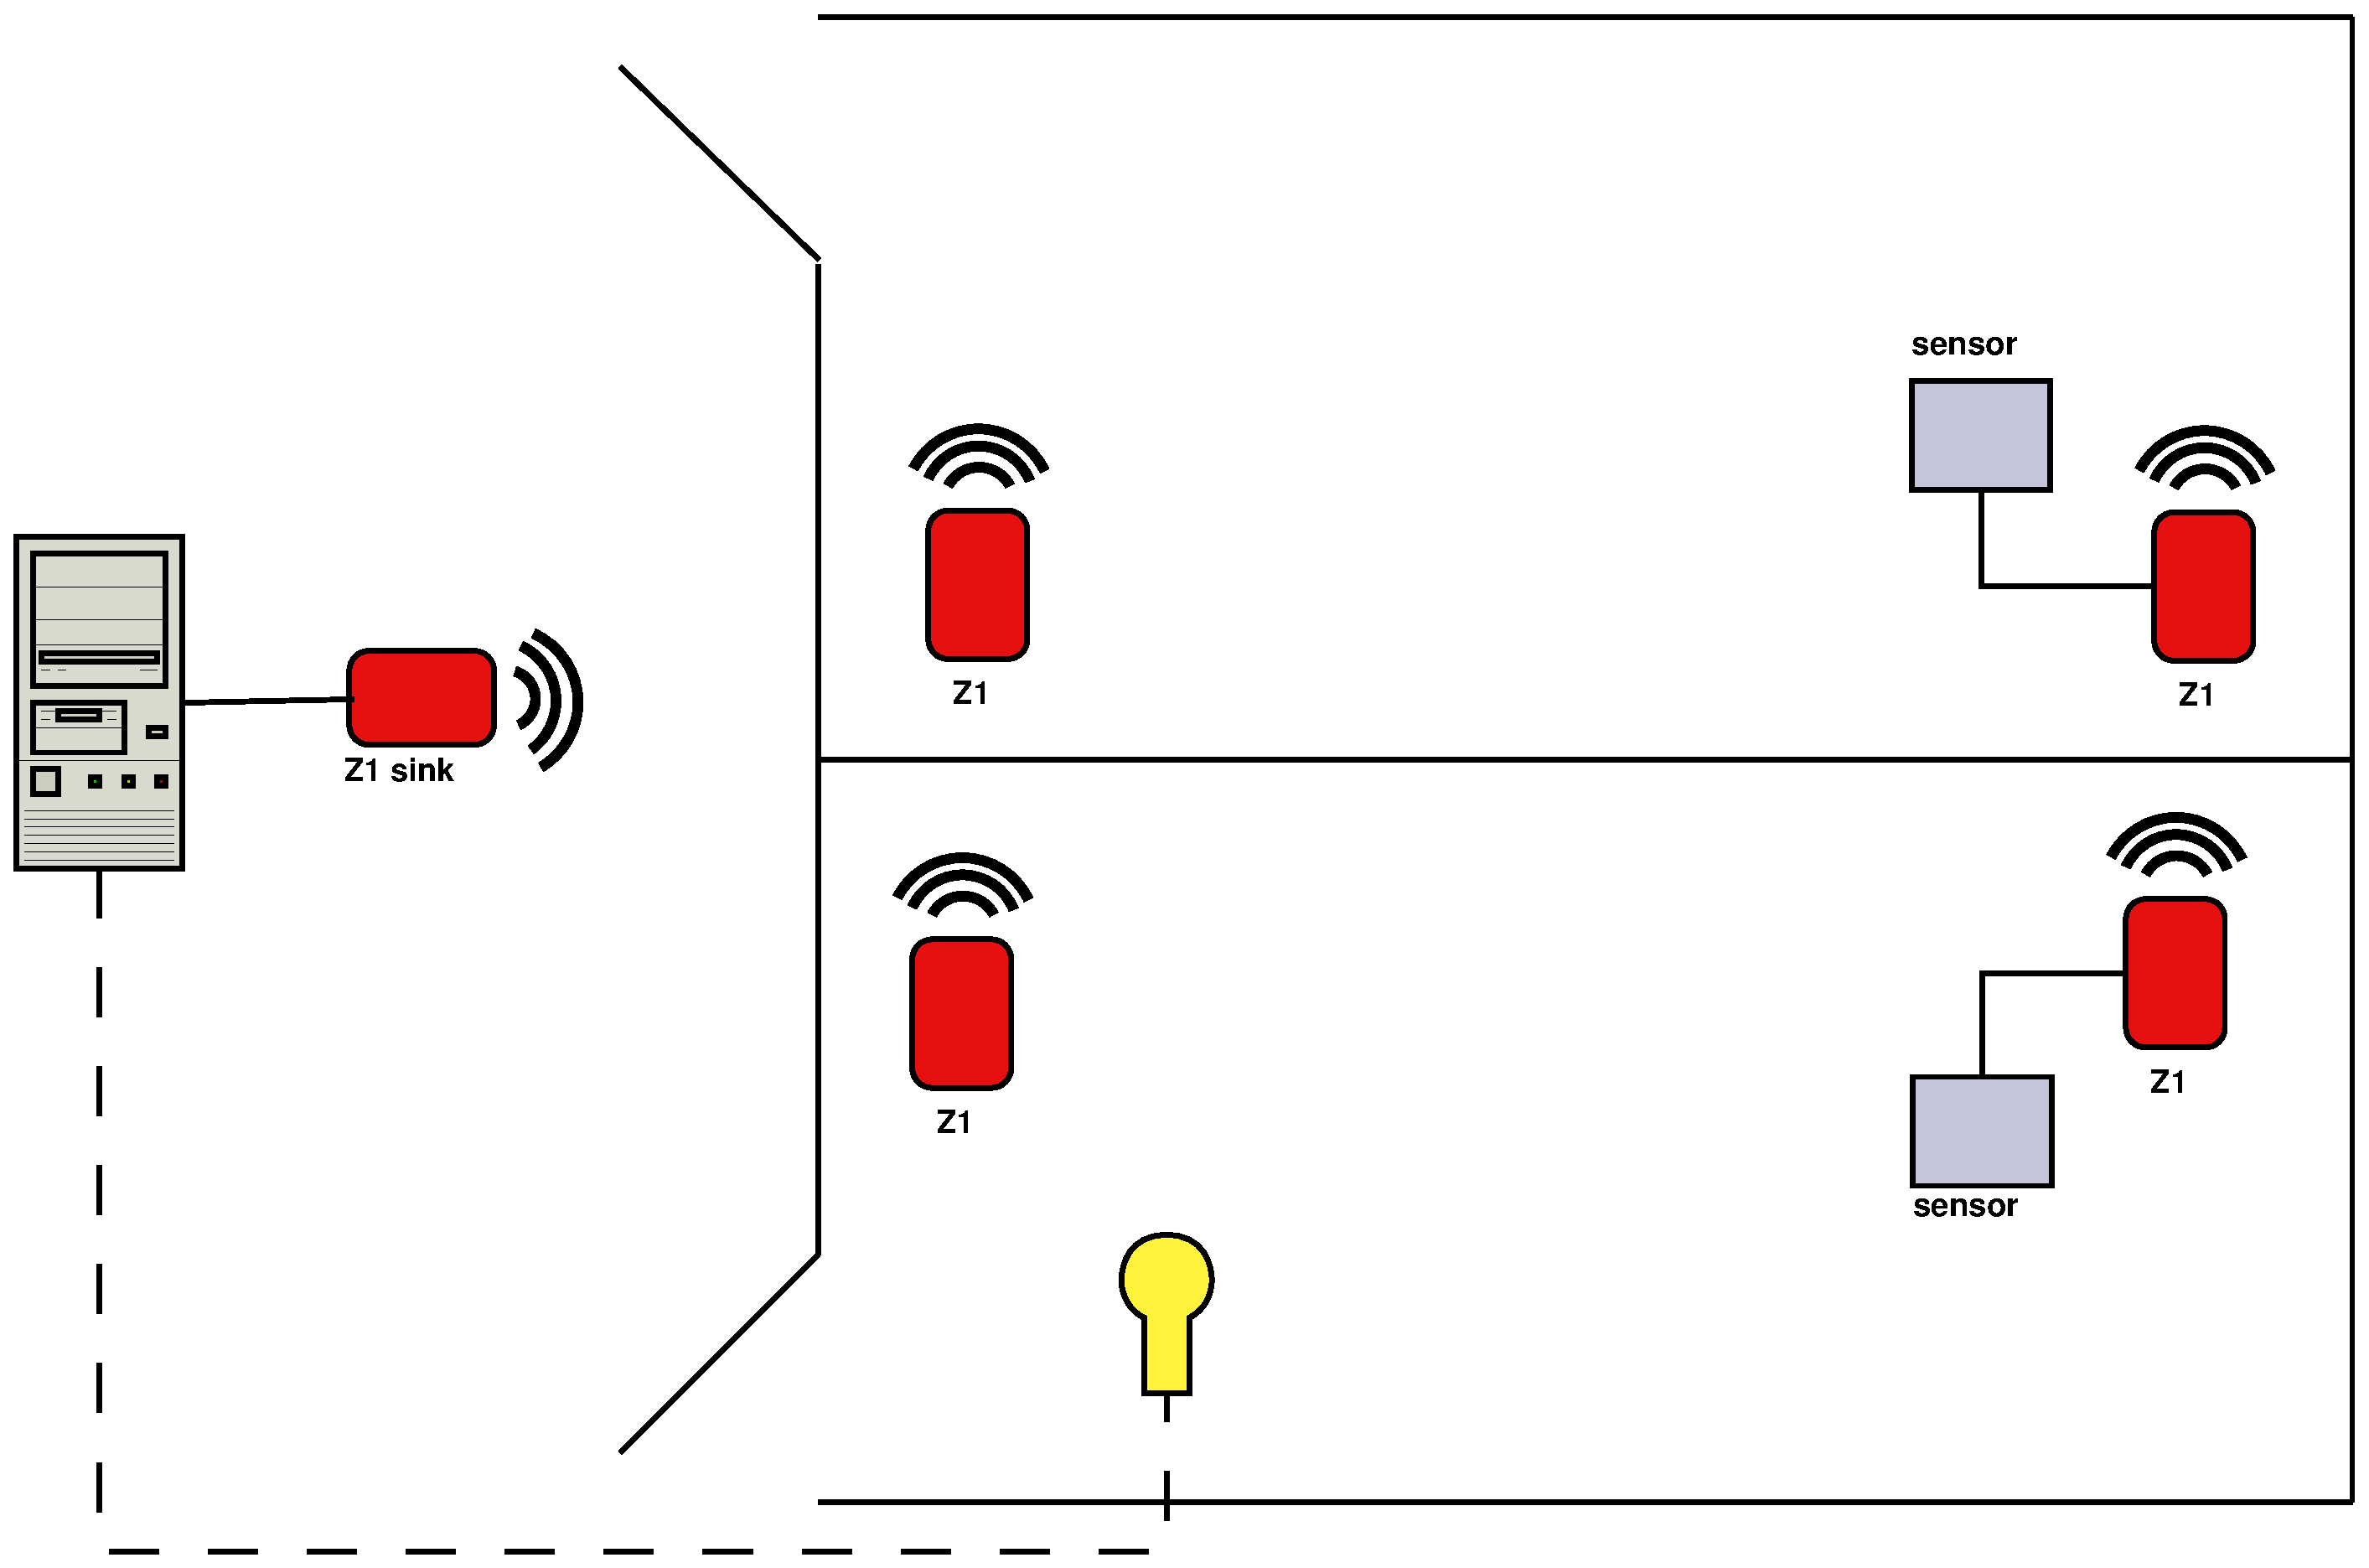
\includegraphics[width=\textwidth]{system.eps}
		\caption{WIPS scenario.}
	\end{figure}
	
\end{frame}

\begin{frame}
\frametitle{Project goals}

	\begin{block}

		\begin{itemize}

			\item
Research existing WSN networking stacks and environmental monitoring techniques.
			\item
Create and implement heuristics for indoor presence sensing.
			\item
Evaluation of different networking solutions and energy efficient MAC protocols.
			\item
Implement and deploy working WSN based on evaluation results.
			\item
Implement data manager and web interface for data presentation.
		
		\end{itemize}

	\end{block}

\end{frame}

\begin{frame}
\frametitle{WSN hardware}

	\begin{columns}

		\column{0.5\textwidth}
	
			\begin{figure}
				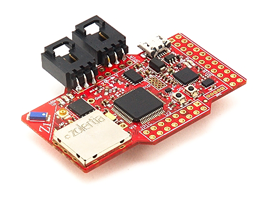
\includegraphics[width=0.5\textwidth]{z1.png}
				\caption{Zolerta Z1 \cite{z1}.}
			\end{figure}

		\column{0.5\textwidth}

			\begin{figure}
				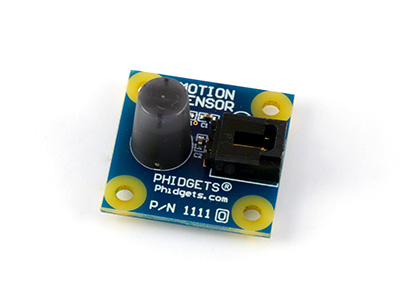
\includegraphics[width=0.5\textwidth]{1111.jpg}
				\caption{Motion Sensor, Phidget 1111 \cite{1111}.}
			\end{figure}

			\begin{figure}
				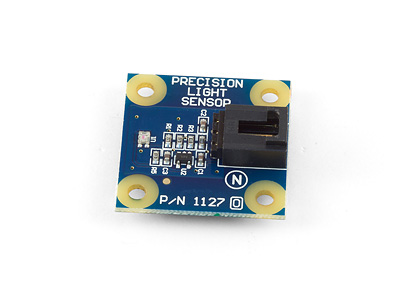
\includegraphics[width=0.5\textwidth]{1127.jpg}
				\caption{Precision Light Sensor, Phidget 1127 \cite{1111}.}
			\end{figure}

	\end{columns}

\end{frame}

\begin{frame}
\frametitle{Home automation hardware}

	\begin{columns}

		\column{0.5\textwidth}
	
		\begin{center}
			\begin{figure}
				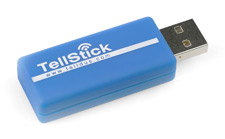
\includegraphics[width=0.5\textwidth]{tellstick.jpg}
				\caption{Telldus Tellstick \cite{tellstick}.}
			\end{figure}
		\end{center}

		\column{0.5\textwidth}

		\begin{center}
			\begin{figure}
				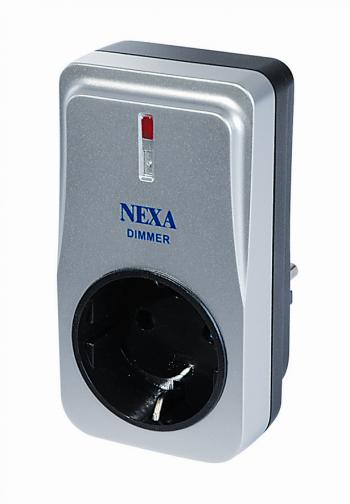
\includegraphics[width=0.5\textwidth]{lycr-300.jpg}
				\caption{Nexa LYCR-300 \cite{lycr-300}.}
			\end{figure}
		\end{center}

	\end{columns}

\end{frame}

\begin{frame}
\frametitle{WIPS system design}

	\begin{center}
		\begin{figure}
			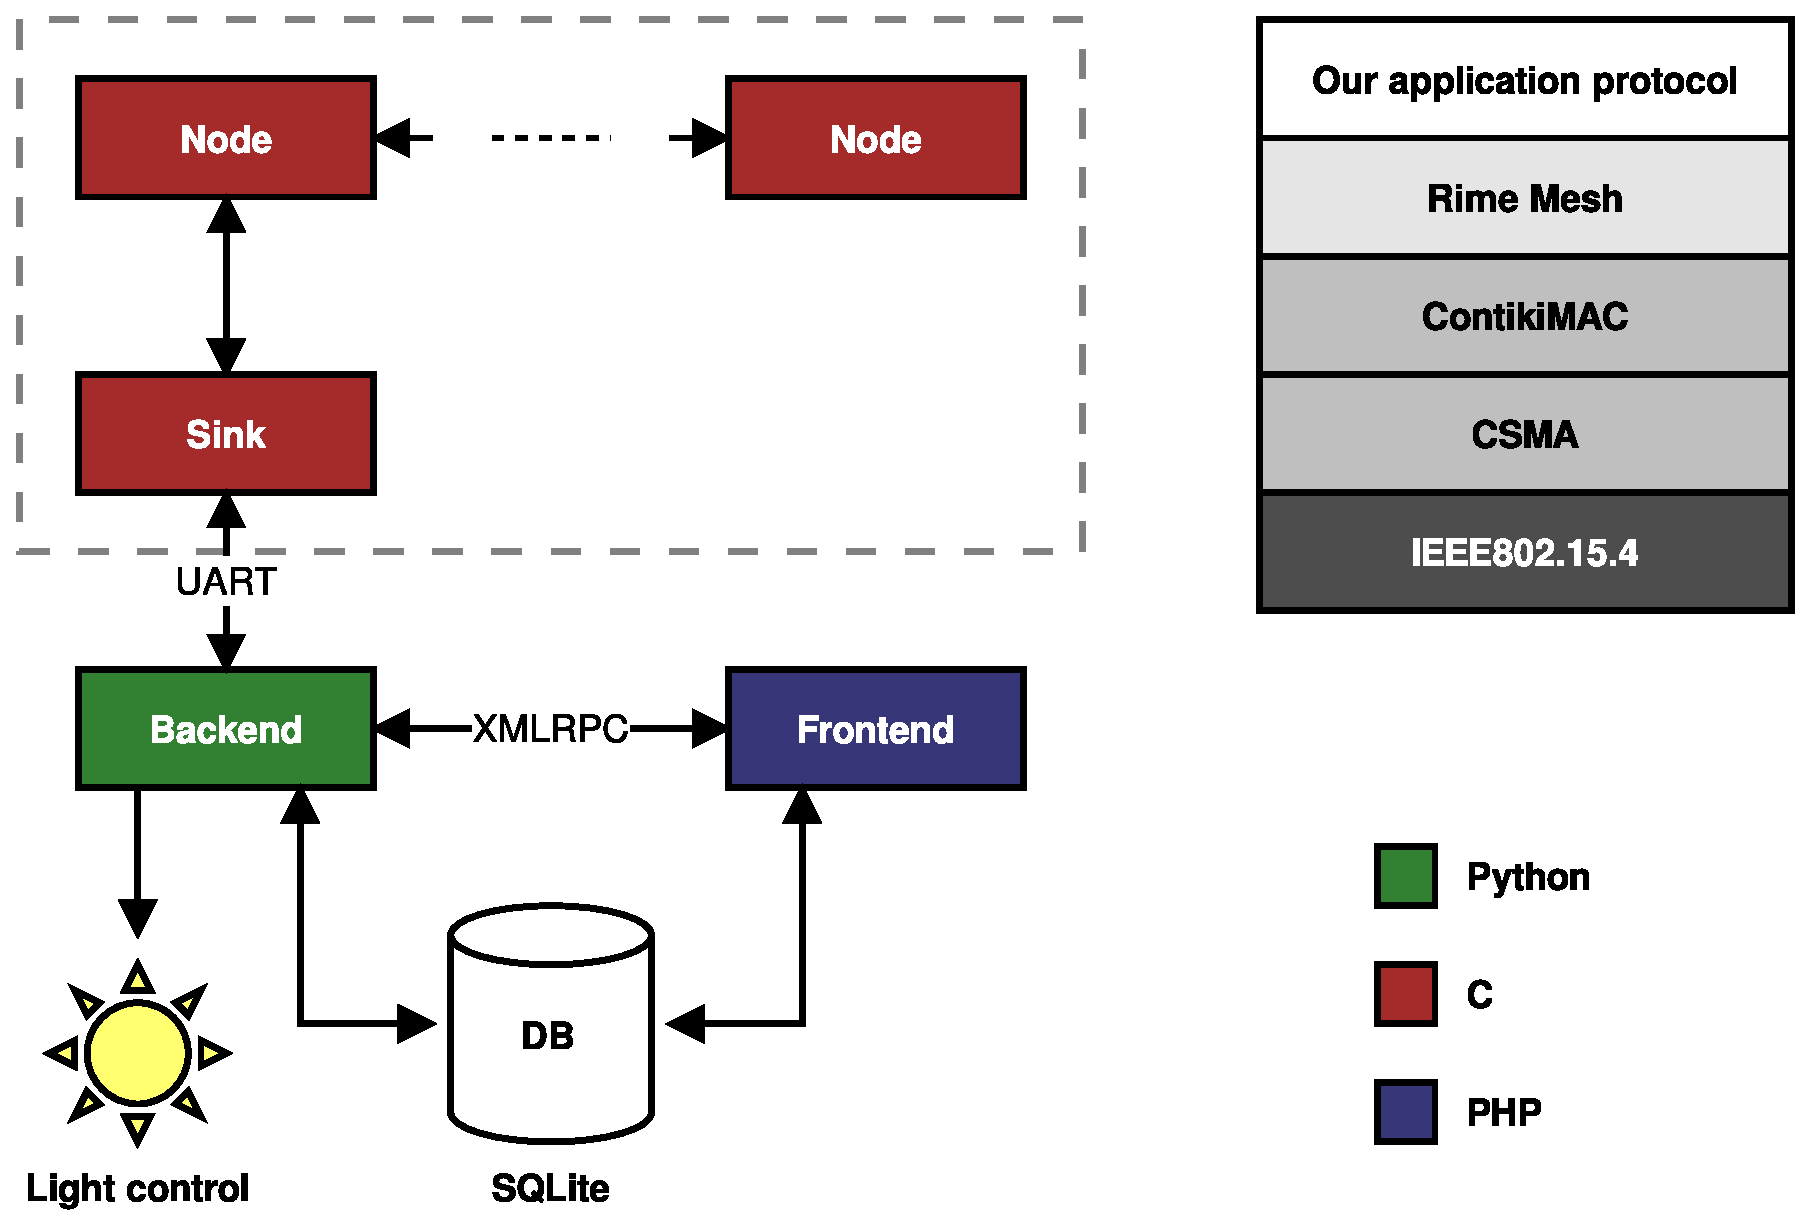
\includegraphics[width=\textwidth]{design.eps}
			\caption{WIPS system design.}
		\end{figure}
	\end{center}

\end{frame}

\begin{frame}
\frametitle{Network evaluation}

	\begin{center}
		\begin{figure}
			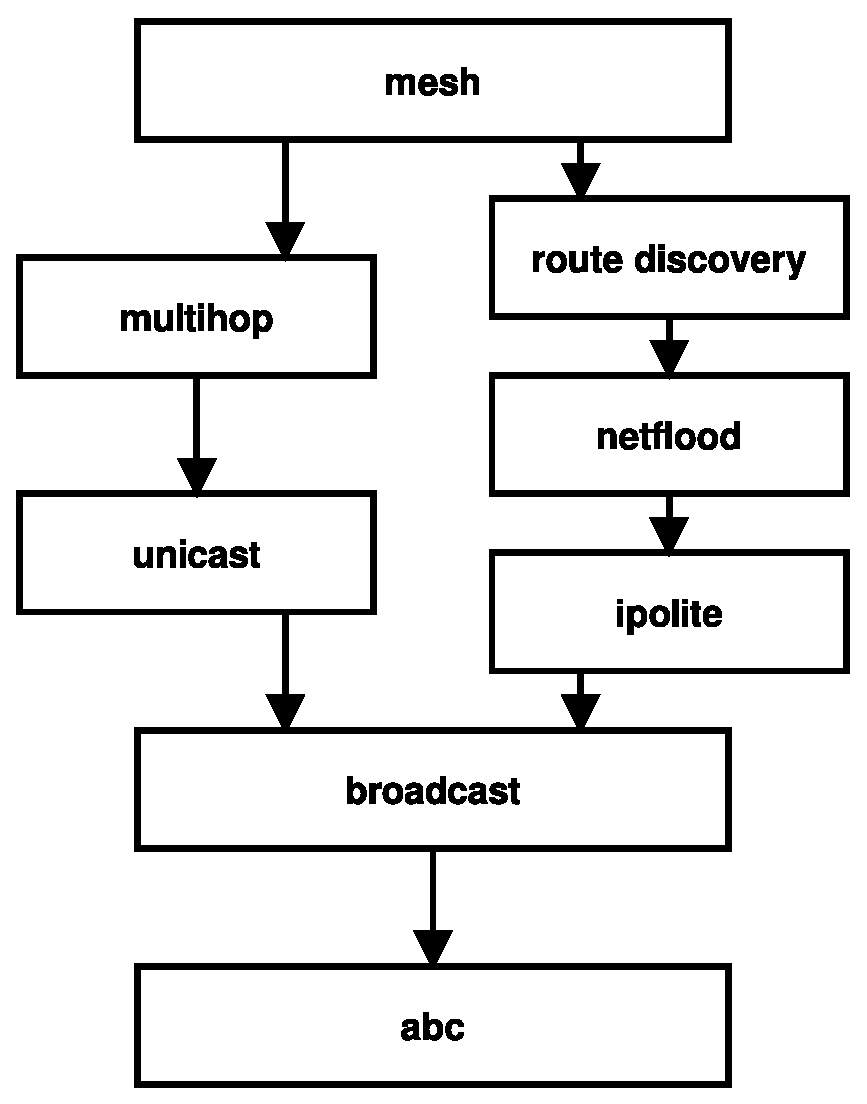
\includegraphics[width=0.5\textwidth]{rimelite.eps}
			\caption{Rime network stack \cite{rime}.}
		\end{figure}
	\end{center}

\end{frame}

\begin{frame}
\frametitle{Mesh example}
	
	\begin{center}
		\begin{figure}
			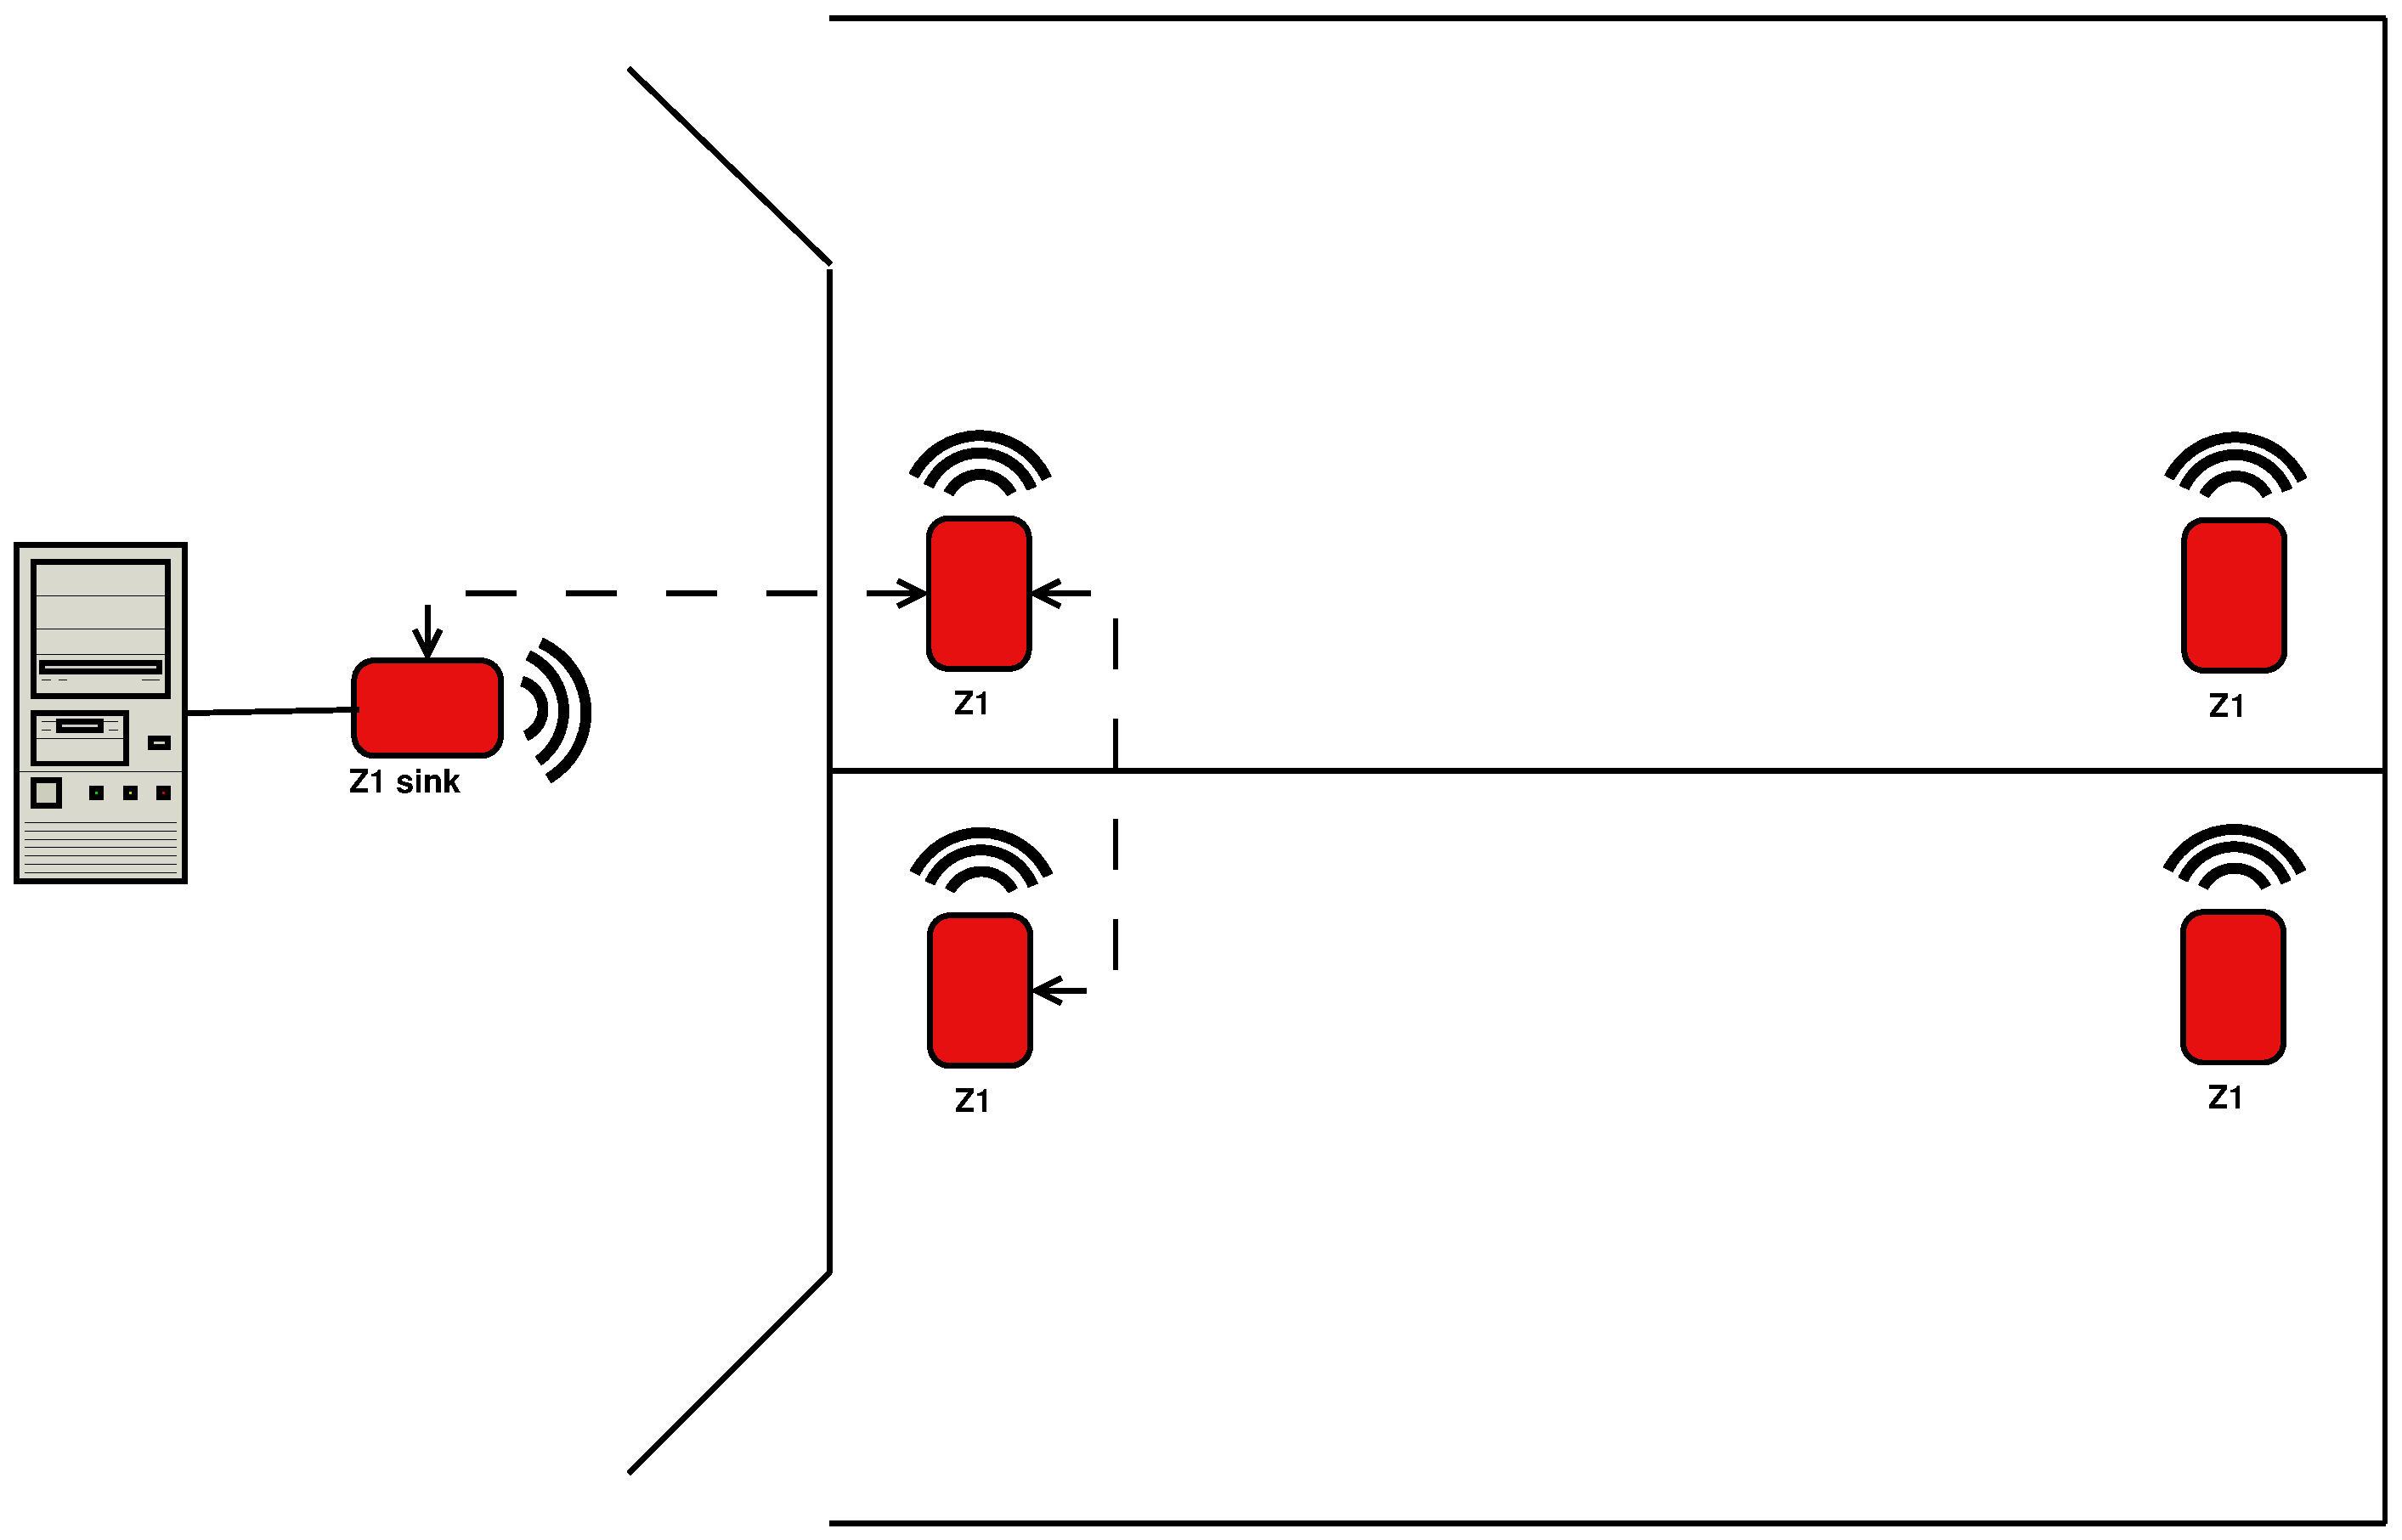
\includegraphics[width=\textwidth]{mesh_example.eps}
			\caption{Mesh example.}
		\end{figure}
	\end{center}
	
\end{frame}

\begin{frame}
\frametitle{Mesh evaluation}
	
	\begin{center}
		\begin{figure}
			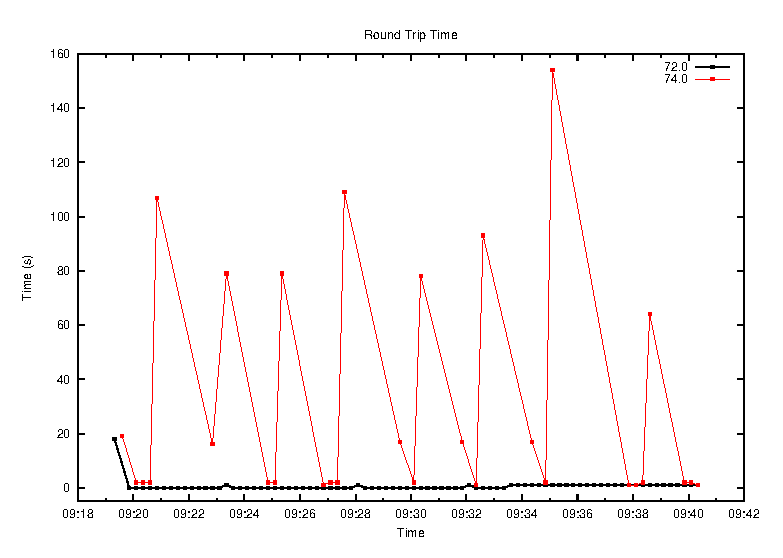
\includegraphics[width=\textwidth]{plot_unpatched.eps}
			\caption{RTT standard mesh.}
		\end{figure}
	\end{center}
	
\end{frame}

\begin{frame}
\frametitle{Mesh evaluation}
	
	\begin{center}
		\begin{figure}
			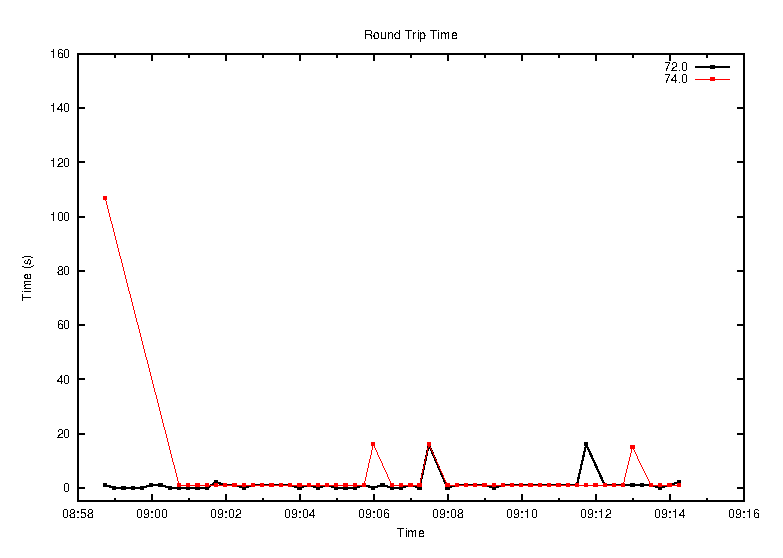
\includegraphics[width=\textwidth]{plot_patched.eps}
			\caption{RTT patched mesh.}
		\end{figure}
	\end{center}
	
\end{frame}

\begin{frame}
\frametitle{Sensor evaluation}

	\begin{center}
		\begin{figure}
			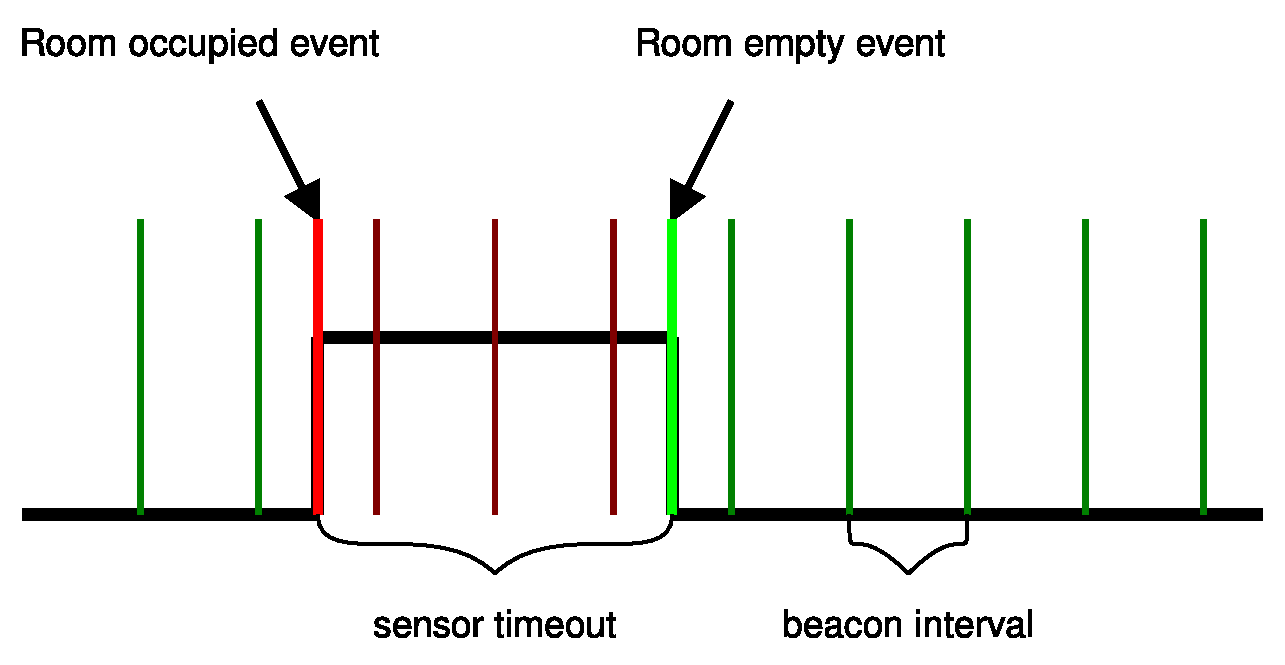
\includegraphics[width=\textwidth]{sensor.eps}
			\caption{Sensor heuristics.}
		\end{figure}
	\end{center}

\end{frame}

\begin{frame}
\frametitle{Protocol implementation}

	\begin{center}
		\begin{figure}
			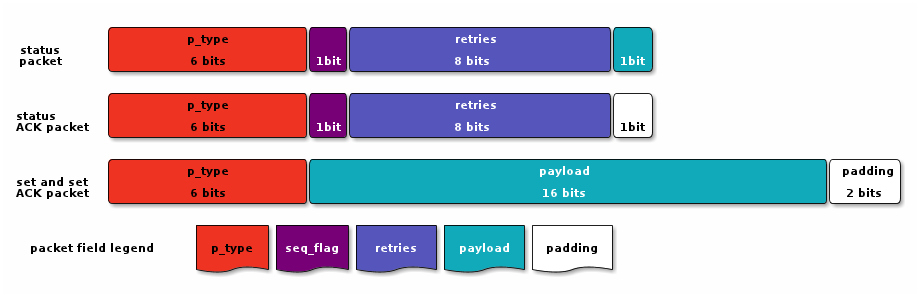
\includegraphics[width=\textwidth]{packet.png}
			\caption{Packet headers.}
		\end{figure}
	\end{center}
	
\end{frame}

\begin{frame}
\frametitle{DB backend}

	\begin{center}
		\begin{figure}
			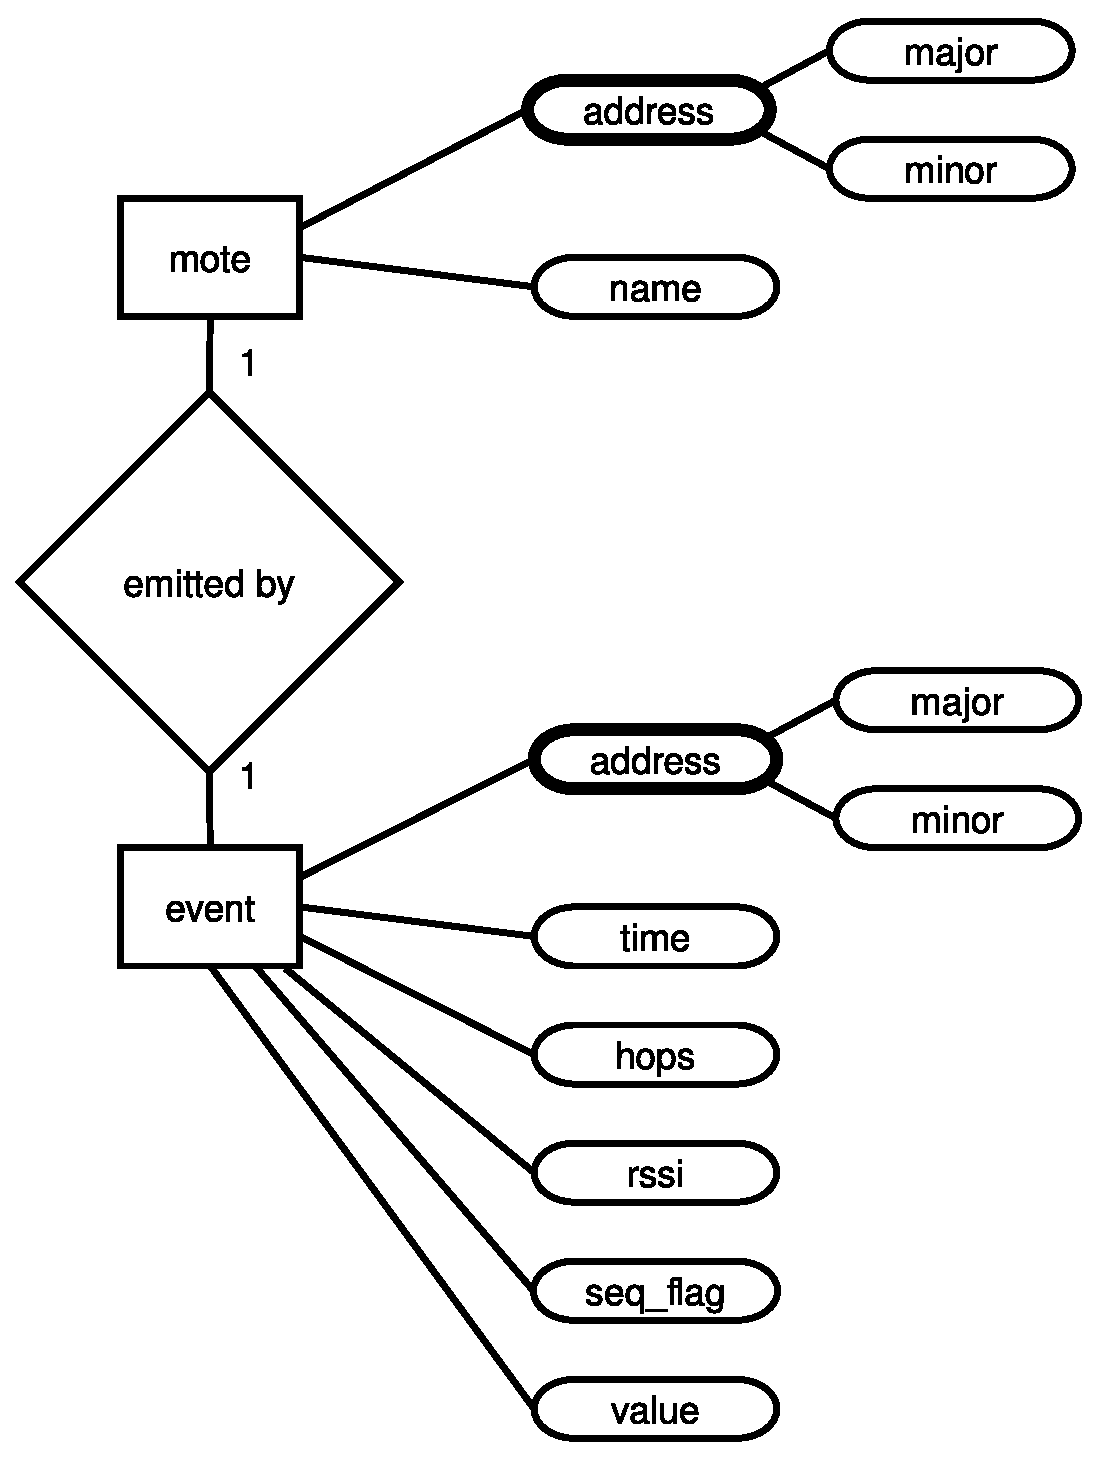
\includegraphics[width=0.5\textwidth]{dbbackend.eps}
			\caption{DB backend.}
		\end{figure}
	\end{center}

\end{frame}

\begin{frame}
\frametitle{Web frontend}

	\begin{center}
		\begin{figure}
			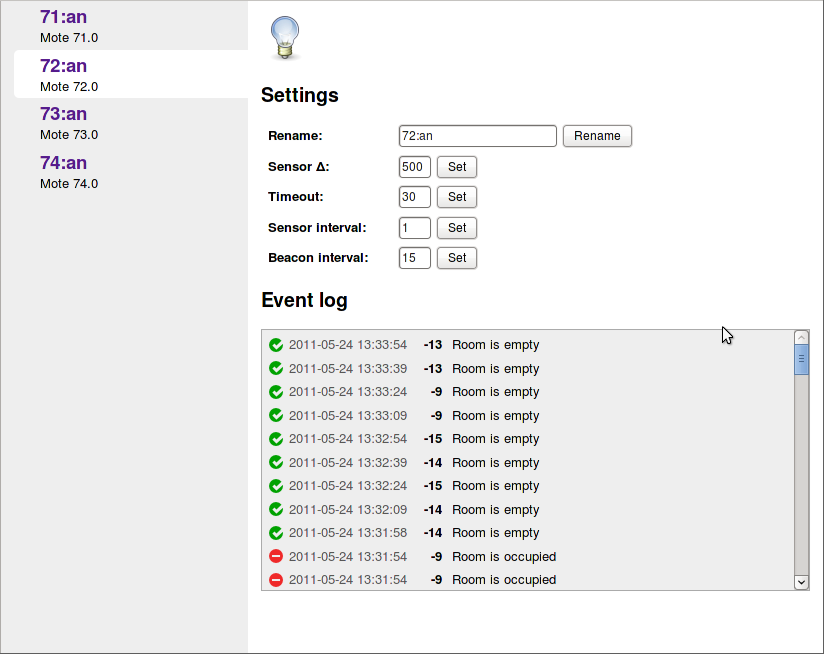
\includegraphics[width=0.75\textwidth]{webfrontend.png}
			\caption{Web frontend.}
		\end{figure}
	\end{center}

\end{frame}

\begin{frame}
\frametitle{Results}

	\begin{block}
		
		Network evaluation and implementation.

	\end{block}	
	
	\begin{block}
				
		Sensor evaluation and implementation.
		
	\end{block}
		
	\begin{block}
		
		Message protocol.
		
	\end{block}

	\begin{block}
		
		Glue code.

	\end{block}

\end{frame}

\begin{frame}
\frametitle{DEMO}
	
	DEMO
	
\end{frame}

\begin{frame}
\frametitle{References}

\begin{thebibliography}{10} 

\bibitem{rime}
An Adaptive Communication Architecture for Wireless Sensor Networks
\newblock Adam Dunkels, Fredrik Österlind, Zhitao He

\bibitem{z1}
Zolertia Z1.
\newblock \url{http://zolertia.sourceforge.net/wiki/images/4/4f/Z1-B-medium.png}

\bibitem{1111}
Motion Sensor, Phidget 1111.
\newblock \url{http://www.phidgets.com/images/1111.jpg}

\bibitem{1127}
Precision Light Sensor, Phidget 1127.
\newblock \url{http://www.phidgets.com/images/1127.jpg}

\bibitem{tellstick}
Telldus Tellstick.
\newblock \url{http://www.evermedia.se/media/5984/tellstick.jpg}

\bibitem{lycr-300}
NEXA LYCR-300.
\newblock \url{http://www.nexa.se/res/produktbilder_stora/lyc_dimmer.jpg}

\end{thebibliography}

\end{frame}

\end{document}